%!BIB program = bibtex
\documentclass[9pt, twocolumn, twoside, lineno]{pnas-new}
% Use the lineno option to display guide line numbers if required.

% PNAS研究论文模板
\templatetype{pnasresearcharticle} % Choose template 
% {pnasresearcharticle} = Template for a two-column research article
% {pnasmathematics} %= Template for a one-column mathematics article
% {pnasinvited} %= Template for a PNAS invited submission
% \usepackage{cite}
\usepackage{url}	
% 文章标题:“流域尺度的水资源利用体系:过渡框架和发展困局”
\title{Identifying regime transitions for water governance at a basin scale}
\label{title}
% Use letters for affiliations, numbers to show equal authorship (if applicable) and to indicate the corresponding author
% 作者列表
\author[a, b]{Shuang Song}  % 宋爽,一作
\author[a, b]{Shuai Wang}  % 王老师,通讯
\author[c, d]{Xutong Wu}  % 武旭同
\author[e]{Yongping Wei} % 尉老师
\author[f]{Graeme S. Cumming} % Cumming
\author[a, b, 1]{Bojie Fu}  % 傅老师

% 机构列表
\affil[a]{ % 北师大地表国重
	State Key Laboratory of Earth Surface Processes and Resource Ecology, 
	Faculty of Geographical Science, 
	Beijing Normal University, 
	Beijing 100875, 
	P.R. China
}
\affil[b]{ % 北师大地理学部
	Institute of Land Surface System and Sustainability, 
	Faculty of Geographical Science, 
	Beijing Normal University, 
	Beijing 100875, 
	P.R. China
}
\affil[c]{ % 北大城环
	College of Urban and Environmental Sciences, 
	Peking University, 
	Beijing 100871, 
	P.R. China
}
\affil[d]{ % 中科院生态中心
	State Key Laboratory of Urban and Regional Ecology, 
	Research Center for Eco-Environmental Sciences, 
	Chinese Academy of Sciences, 
	Beijing 100085, 
	P.R. China 
}
\affil[e]{ % 昆士兰大学
	School of Earth and Environmental Sciences, 
	The University of Queensland, 
	Brisbane 4067, 
	Australia
}
\affil[f]{
	ARC Centre of Excellence for Coral Reef Studies, 
	James Cook University, 
	Townsville 4811, 
	QLD, Australia
}

% Please give the surname of the lead author for the running footer
% 领衔作者
\leadauthor{Song} 

% Please add a significance statement to explain the relevance of your work
% PNAS特有的“Significance陈述”,用不超过120个字来说明研究的意义和亮点
\significancestatement{
\label{significance}
	% Authors must submit a 120-word maximum statement about the significance of their research paper written at a level understandable to an undergraduate educated scientist outside their field of speciality. The primary goal of the significance statement is to explain the relevance of the work in broad context to a broad readership. The significance statement appears in the paper itself and is required for all research papers.
	% 人类社会的发展和维持依赖于水。由于自然水循环被加速的社会经济过程推向水社会水循环,大的河流流域往往被控制阶段进一步用水。
	Development and maintenance of human societies depends on water. As natural water cycles are pushed by accelerating socio-economic processes towards a hydrosocial water cycle, big river basins are often governed phase by phase for further water use. We propose an integrated index to detect water governance regimes and apply it to the Yellow River Basin, a fast-changing basin. Three water governance regimes are identified (massive supply, purpose-focused, and many-sided governance). They suggest a general regime-transition schema for large river basins. By linking river basin governance transitions with major water governance challenges, our approach can offer useful sustainability guidelines for big river basins all around the world.
}

% Please include corresponding author, author contribution and author declaration information
\authorcontributions{ % 作者的相应贡献
	Shuai Wang and Bojie Fu designed this research,
	Shuang Song performed the research and analysed data,
	Shuang Song, Xutong Wu wrote the paper.
	Yongping Wei and Graeme S. Cumming reviewed the manuscript and proposed major useful advices.
}
\authordeclaration{ % 利益冲突陈述
	The authors declare no competing interests.
}

% 如果有共同一作的情况,则uncomment下面这行代码的注释
%\equalauthors{\textsuperscript{1}A.O.(Author One) contributed equally to this work with A.T. (Author Two) (remove if not applicable).}

% 通讯作者信息
\correspondingauthor{\textsuperscript{1}To whom correspondence should be addressed. E-mail: bfu@rcees.ac.cn}

% 关键词,三到五个
% At least three keywords are required at submission. Please provide three to five keywords, separated by the pipe symbol.
\keywords{Regime shifts $|$ Water use $|$ Water governance $|$ Transformation $|$ Sustainability} 

%tag 摘要
% 为了
\begin{abstract}
	\label{abstract}
	In many large river basins, the use and governance of rivers for socio-economic development has led to a global transformation from natural to social-ecological or ‘hydrosocial’ water regimes. Water governance decides who gets water, when, and how much. Identifying how and when water governance regimes change is therefore critical to understanding social-ecological water dynamics and guiding the efficient and sustainable use of water. We combined three main dimensions of water governance (supply, purpose and allocation) to develop a quantitative Integrated Water Governance Index (IWGI) that can detect regime shifts in water governance at a basin scale. Applying the index to a rapidly-changing large river basin (the Yellow River Basin, China) shows that it can describe shifts between three water governance regimes (respectively, massive supply regime; purpose-focused regime; and many-sided governance regime) over half a century, and offer a way to relate these shifts to environmental, economic social and political changes. Our application of the IWGI suggests a widespread transition schema for water governance regimes and a general transformative trajectory as a hypothesis for understanding hydrosocial water cycles in the Anthropocene. The different governance challenges that occurred at different phases of the transition of the Yellow River also suggest potentially useful guidelines for the coordinated governance of big river basins in general.
\end{abstract}


\dates{This manuscript was compiled on \today}
\doi{\url{www.pnas.org/cgi/doi/10.1073/pnas.XXXXXXXXXX}}


\begin{document}

\maketitle
\thispagestyle{firststyle}
\ifthenelse{\boolean{shortarticle}}{\ifthenelse{\boolean{singlecolumn}}{\abscontentformatted}{\abscontent}}{}
% If your first paragraph (i.e. with the \dropcap) contains a list environment (quote, quotation, theorem, definition, enumerate, itemize...), the line after the list may have some extra indentation. If this is the case, add \parshape=0 to the end of the list environment.

\label{introduction-section-1}
% 作为“人类世行星戏剧的中心”, water 不仅对地球系统进程至关重要,而且还支持着人类社会的发展。
\dropcap{W}ater has been described as being “at the centre of the planetary drama of the Anthropocene” \cite{gleeson2020}.
% 由于人类对水的依赖,人类活动深刻地改变了自然水循环,并逐步走向水-社会水循环。
It is essential, not only for earth system processes but also in supporting the economic development and continued wellbeing of human societies. Human activities stemming from our reliance on water have profoundly modified the natural water cycle, moving rivers along a trajectory towards a hydrosocial water cycle
\cite{gleeson2020,sivapalanSociohydrologynewscience2012,qin2014,abbottwatercycleAnthropocene2019,levia2020}, in which social and power relations dominate the nature of hydrological cycles.
% 面对这一重大转型,世界上许多大流域作为经济和文明热点,迫切需要成功的可持续治理
Facing this major transformation, many of the world’s big river basins (which are hot spots of civilization and economic growth) are urgently in need of new models of water governance for sustainability
\cite{bestAnthropogenicStressesWorld2019,falkenmark2019,dibaldassarreSociohydrologyScientificChallenges2019}. 
% 水治理作为地球系统治理框架的重要组成部分,需要对人与水之间复杂的关系有深刻的理解。
As an integral part of a proposed earth system governance framework, sustainable water governance requires a deep understanding of the complex relationships between people and water
\cite{biermann2012,steffen2020,dibaldassarreSociohydrologyScientificChallenges2019}.

\label{introduction-section-2}
% 缺乏治理就是缺乏可持续性
For water resources in populated areas, missing governance means missing sustainability \cite{undpwatergovernancefacility2015}.
% 确定向社会水循环过渡的第一个重要步骤是确定发生过渡的不同制度。
A first important step in identifying transitions towards a hydrosocial water cycle is to identify the different regimes under which it occurs.
% 根据联合国开发计划署(UNDP)的说法,水管理决定了用水的三个关键方面:“有多少水可供使用?、“如何平衡用水服务?”“以及‘如何平等有效地分配水资源?’”
According to the United Nations Development Programme (UNDP), three key dimensions of water use are decided by the water governance regime directly: ``How much water can be used?'' (supply), ``How can different services provided by water be balanced?'' (purpose), and ``How can water be allocated equally and efficiently?'' (allocation)
\cite{undpwatergovernancefacility2013,undpwatergovernancefacility2015,undpwatergovernancefacility2016}.
% 制度是系统结构和功能的一种稳定状态,其大规模的持续变化可能对系统结果产生实质性的影响,具有广泛的级联效应,即制度变迁.
A regime is defined as a locally stable state of a system’s structure, function, and dominant controls \cite{carpenterEarlyWarningsRegime2011}. 
Large and persistent changes in key system properties may lead to a loss of local stability, potentially resulting in a regime shift with impacts on system outcomes and widespread cascading effects
\cite{rocha2018,gregr2020}.
% 因此,制度的转变是水治理发生实质性变化的信号,可能导致对可持续性的新挑战。
Regime shifts are both consequences and signals of substantive changes in water governance, and may lead to new challenges to sustainability.

% 除了由关键的环境、经济、社会和政治变量的变化引起外,水治理的制度变迁也可以通过治理的三个关键维度(供应、目的和分配)
In addition to being caused by changes in key environmental, economic, social and political variables, regime shifts in water governance can be triggered through changes in each of the three key dimensions of governance (supply, purpose, and allocation) 
\cite{undpwatergovernancefacility2013,undpwatergovernancefacility2015,undpwatergovernancefacility2016}.
% 首先,水的供应不仅取决于天气(许多地区的长期趋势令人担忧,如冰川的消失),还取决于诸如灌溉和工业等经济活动的需求;蓄水可以解决部分问题,但不能解决所有问题
First, the supply of water depends not only on weather (with worrying long-term trends in many regions, such as the loss of glaciers) but also on the demands of economic activities such as irrigation and industry; water storage can resolve some but not all of these issues 
\cite{greveGlobalAssessmentWater2018, wada2017,qinFlexibilityintensityglobal2019}.
% 其次,在供应用水(如家庭用水和粮食生产用水)和非供应用水(如工业生产或能源用水)之间存在权衡,这需要由治理制度来平衡。
Second, the purposes for which water is used are in need of balanced between consumptive uses (e.g., drinking and food production) and non-consumptive uses (e.g., energy production or urban services)  
\cite{liu2017, florke2018,kleemannQuantifyinginterregionalflows2020}.
% 水治理可以看作是为每一个不同的目的分配权重并执行结果规则的过程。
Water governance can be viewed as the process of assigning weights to each of these different purposes and enforcing the resulting rules.
% 第三,由于配置是流域关注的问题,它不仅受到区域环境基础的影响,而且还受到区域经济比较优势的影响,而经济比较优势可能受到社会发展和政策的影响。
Third, the allocation of water across the whole basin is influenced not only by regional environmental context but also by local socio-economic trends and regions’ comparative economic advantages, which can be altered by changing social and political drivers
\cite{roobavannan2017,speed2013}.
% 综上所述,随着向以人为主导的水-社会水循环的转变,水治理制度由三个变化的维度(供应、目的和分配)决定,缺乏简单而全面的方法来确定制度变化,这对成功治理留下了关键的差距.
Despite the obvious relevance of substantive changes in any of the three dimensions of water governance, the lack of a simple but comprehensive method for identifying changes in water governance regimes makes it difficult to achieve water governance for sustainability (Figure~\ref{fig:framework}).

\label{introduction-section-3}
% 黄河流域(YRB,详见方法S2)经历了中国最密集的用水和剧烈的制度变迁,从古代起就面临着水资源管理方面的非凡挑战。
As an informative example, we focus on the Yellow River Basin (YRB, see \textit{Appendix} Methods S1 and Figure S1 for details). 
The YRB has experienced some of the most intense water use and dramatic regime shifts of any large river basin in China, giving rise to long-standing challenges for its governance.
% 半个世纪前,黄河巨大的泥沙负荷不仅给黄河带来了灾难,也给黄河的用水带来了困难。
From about 550BC until half a century ago, flooding and the huge sediment loads of the Yellow River brought frequent human disasters and the constant shifts in the river’s channel made it difficult for people to use its waters 
\cite{songSedimenttransportincreasing2020a,li2020}. 
% 自20世纪60年代以来,通过实施养护措施、水库调蓄和堤防工程,这些问题得到了有效遏制。
Since the 1960s, the implementation of conservation measures, regulation reservoirs, and levee constructions have contained the issues caused by high-sediment loads
\cite{wangReducedsedimenttransport2016,wu2020}.
% 然而,由于过度用水,黄河的严重干涸带来了新的治理挑战,并推动了一系列相关政策(如调节用水和限制取水)来应对。
However, water over-use has led to drying up of the Yellow River, creating new governance challenges that have been addressed through a range of related policies (e.g., regulating water use and limiting water withdrawals) 
\cite{xia2012}.
% 今天,由于水的需求仍然难以完全满足,各区域和部门之间必须进行各种权衡,要取得成功的水治理还有很长的路要走。
Today, given that it is still difficult to completely meet water demands and various trade-offs must be negotiated between regions and sectors, there is still a long way to go towards successful water governance 
\cite{wangYellowRiverwater2019,wohlfartSocialecologicalchallenges2016}.
% 总而言之,YRB是世界上变化最迅速的盆地,对由环境、经济、社会或政治因素引起的无休止的治理挑战作出各种各样的反应。
All in all, the YRB has been among the most rapidly-changing large river basins in the world, with myriad responses to the endless governance challenges induced by environmental, economic, social and political factors. 
% 因此,确定长江流域水资源管理制度的变化可以为了解世界上快速变化的大流域以及治理如何应对其可持续性挑战提供重要的见解。
Identifying regime shifts in water governance within the YRB can thus provide crucial insights into the world’s rapidly-changing big river basins and the ways in which governance may respond to meeting challenges to their sustainability.

\label{introduction-section-3}
% tag 引言最后一段
% 这里我们整合了三个方向,提出了描绘流域人水关系的指数
We first use the three key dimensions (supply, purpose and allocation) of water governance to develop an Integrated Water Governance Index (IWGI) that can detect and describe changes in water governance at a basin scale (see Figure~\ref{fig:framework} and methods).
% 使用案例研究
Then, by applying the index to a typical rapid-changing big river basin (the YRB), we show how the index can be used to analyse the complicated regimes of water governance and their main causes in a comprehensive but simple way. 
% 最后总结出一般性框架
Finally, we propose a general regime transition scheme as a practical guideline for a coordinated approach to exploring the challenges faced by big river basin governance.


\begin{figure*}%[htbp]
	\centering
	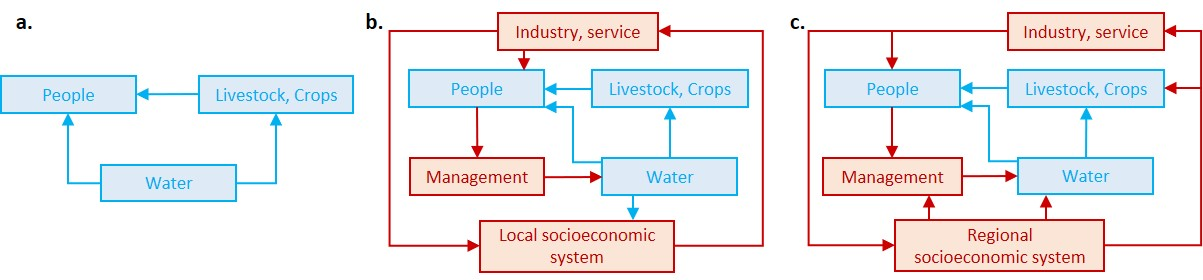
\includegraphics[width=0.8\linewidth]{../../figures/main/framework.jpg}
	\caption{
		A framework for understanding the relationship between transitional water governance regimes and eventual transformation to a hydrosocial cycle. A key missing element in current knowledge is an ability to detect regime shifts using a simple and comprehensive index.
		% 图A是水资源利用的三个维度。每个维度都有两个极点(红色字表示),指示水资源利用在该轴上的两个变化方向。
		\textbf{A:} there are three key dimensions (supply, purpose and allocation) of water governance (see Methods for details). Each dimension has two poles (denoted in red) which indicate the two potential directions of changes along that axis: (1) ``supply'' shifts between scarcity and abundance. (2) ``purpose'' is weighted between consumptive services or non-consumptive uses. (3) ``allocation'' changes between balanced or lopsided. 
		% 图B是将三个维度结合后的变化情况。因上述三个维度随着社会发展而不断变化,其组合的水资源利用状态也不同。这个过程中当突变发生时,可能标志着水资源利用发生了稳态转换,因此我们需要一个指标来监测其变化。
		\textbf{B:} governance changes are an emergent outcome of trends across the three dimensions. Water governance status changes along a trajectory towards a hydrosocial water cycle. When abrupt change occurs, it may indicate a regime shift in water governance
		\cite{steffen2018,abbottwatercycleAnthropocene2019,levia2020}.
	}
	\label{fig:framework}
\end{figure*}


\section*{Results}
\subsection*{Water governance regimes}

\begin{figure}[ht!]
	\centering
	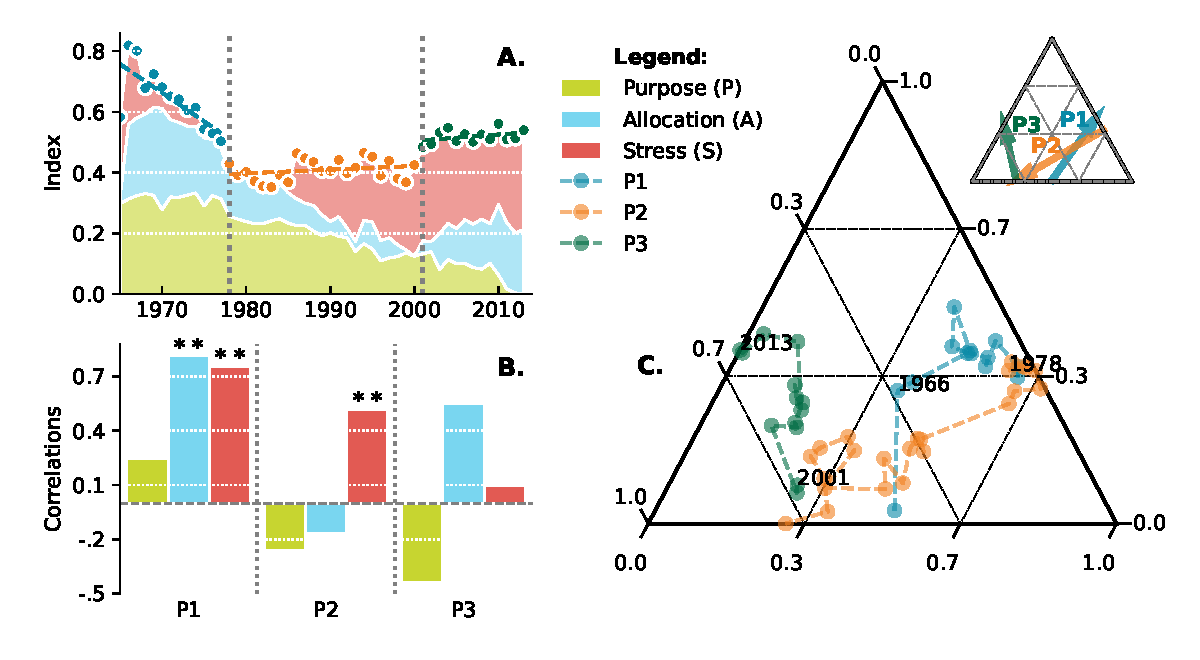
\includegraphics[width=\linewidth]{../../figures/main/index.pdf}
	\caption{Changes in the IWGI index. 
	\textbf{A,} Change points detection. With significant change points in 1978 and 1994, the IWGI has three different periods.
	\textbf{B,} Contributions of each dimension to the changes of IWGI within each of the three periods. Supply, purpose and allocation were respectively the main positive contributors to P1, P2 and P3.
	}
	\label{fig:IWGI}
\end{figure}

% 这一节主要展示IWGI的变化趋势和WUR的划分
With two significant breakpoints, the changes in the IWGI are divided into three periods (Figure~\ref{fig:IWGI}A) with different slopes. 
The changes are contributed by different water governance dimensions (Figure~\ref{fig:IWGI}B).
% 第一阶段
In the first period (P1, 1965-1978), the IWGI increased rapidly. 
Water supply made the most striking positive contribution (131\%), while purpose and allocation had a slight negative contribution (-11\% and -20\%).
% 第二阶段
In the second period (P2, 1979-1994), the contributions of purpose and allocation became positive and the IWGI experienced a drop because steeply declining supply capacity played a larger negative role (dropping to -188\% lower than P1). 
% 第三阶段
In the third period (P3, 1995-2013), as positive contributions from purpose (75\%) and allocation (84\%) increased further and the negative contribution of water supply lessened (-59\%), positive growth of the IWGI returned.

\begin{figure}[!htbp]
	\centering
	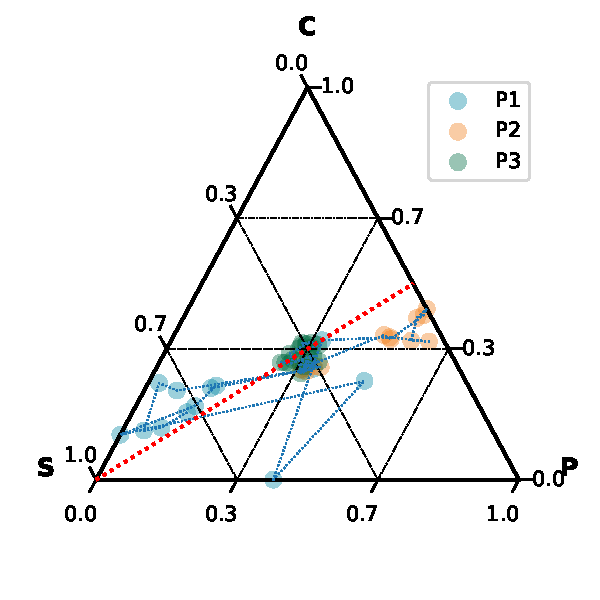
\includegraphics[width=0.9\linewidth]{../../figures/main/phases.pdf}
	\caption{Combination of contributions across three dimensions in different periods (S: supply; P: purpose; A: allocation). The closer a point is to an angle of the outside triangle, the greater the proportion of the contribution of this dimension.
	The red indicator line in this plot denotes a 1:1 contributions between purpose (P) and allocation (A). When the points are below this line, the contribution ratio of allocation is lower than that of function, and \textit{vice versa}.}
	% 由于阶段一的点位于该线上方,L的净贡献比例多于P,而第二阶段的点则恰好相反。
	\label{fig:phases}
\end{figure}

% 每个时期都有一个独特的、最引人注目的、对IWGI作出积极贡献的人。不同时期的三维总体特征如图所示。
Each period has a unique most striking contributor to IWGI in positive. Overall features of the three dimensions in different periods are shown in Figure~\ref{fig:phases}.
% 第一阶段到第二阶段
Throughout P1, the water governance regime was dominated by increasing supply capacities. 
% 第三阶段集中
It then experienced a shift, slowing down in increasing supply during P2, with an accompanying reverse in the contributed proportion between purpose and allocation. Finally, the contribution of all three dimensions was similar in P3 (32.91\%, 31.87\% and 35.21\% for purpose, allocation and supply respectively), making the points cluster at the centre of the diagram. 
% 总结来说,三个稳态
The three different periods corresponded to three distinct water governance regimes: a massive supply regime (P1: 1965-1978), a purpose-focused regime (P2: 1979-1993), and a many-sided governance regime (P3: 1994-2013). 

% tag 结果2
\subsection*{Causes of water governance regime shifts}
\label{result2}

\begin{figure}[th!]
	\centering
	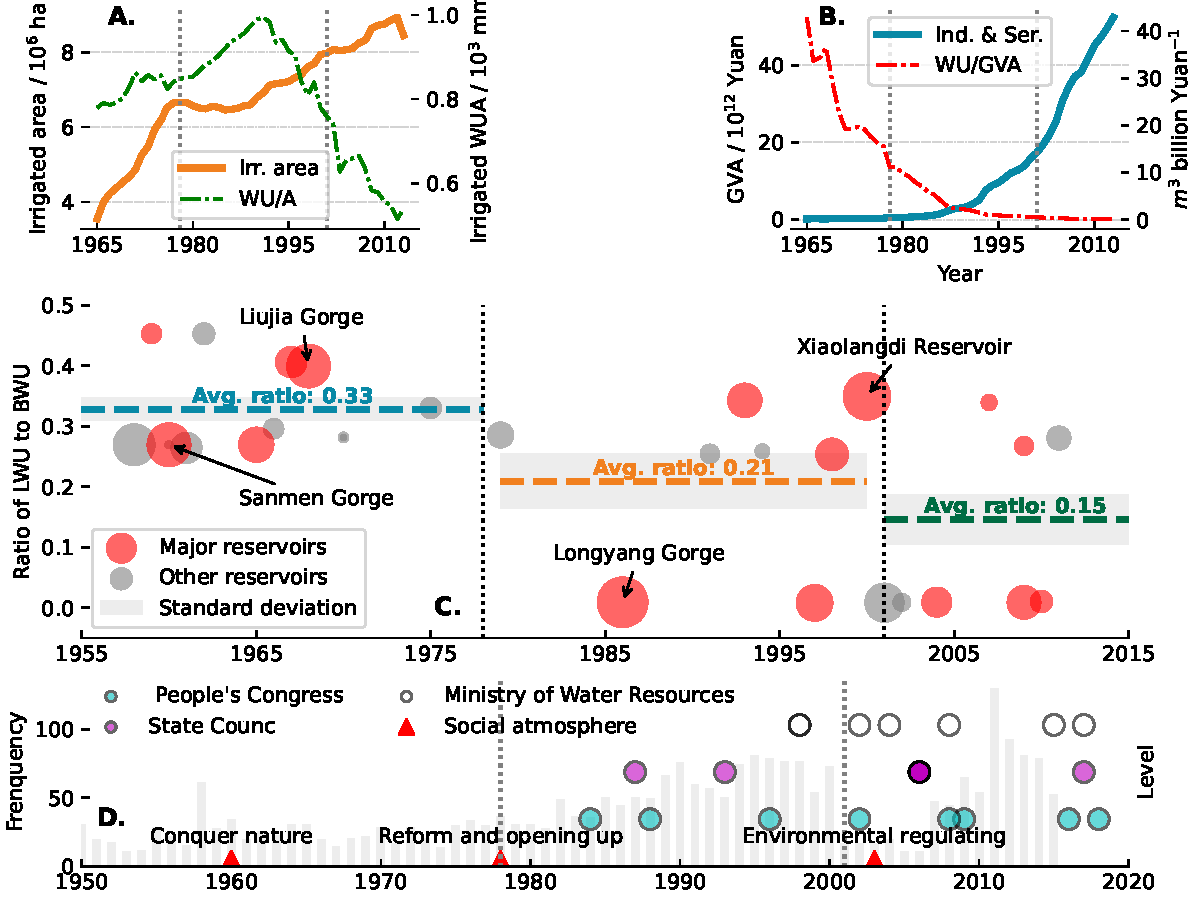
\includegraphics[width=\linewidth]{../../figures/main/causes.pdf}
	\caption{
		Causes of water governance regime shifts in the Yellow River Basin: environmental change, economic growth and efficiency changes, social transformation, and water governance policies.
		\textbf{A.} Changes in total irrigated area (orange line), and water uses in per unit of area (WU/A, green dot line, see \textit{SI Appendix} Methods S2).
		\textbf{B.} Changes in gross values added (GVA) of industry and services (blue line), and their water use for unit production (WU/GVA, red dot line) respectively (\textit{SI Appendix} Methods S2).
		\textbf{C.} Completed time of each new reservoir and their surrounding region's water use percentages as a proportion of the basin's total water use (WU) at that time. Red circles denote hub reservoirs in the basin, which play a role in integrated basin water management. 
		The size of each circle indicates the magnitude of its water storage capacity. Some important reservoirs include: (1) Xiaolangdi reservoir and Sanmen Reservoir, which were constructed mainly for managing sediments; and (2) Impoundments at Liujia Gorge, Longyang Gorge, which were constructed mainly for managing flood water discharge and water supply. The named reservoirs are significant for the entire basin, not only for regional development.
		\textbf{D.} Social transformations and national-level policies related to water governance (see \textit{SI Appendix} Methods S1 and Table S2). In order, the four transformations are ``ethos of conquer nature (since 1958)'', ``reform and opening-up (since 1978)'', ``the 87 Water Allocation Scheme (since 1987)'', ``environmental regulation (since 2003)'' in order (see \textit{SI Appendix} Methods S1).
	}
	\label{fig:Causes}
\end{figure}

% 进一步挖掘IWGI变化的根本原因,灌溉区扩张和工业和服务业的经济增长是P1和P2目的变化的关键。
Digging more deeply into the underlying causes of changes in the IWGI, the expansion of irrigated area and the economic growth of industry and services were key to the change in purpose between P1 and P2. 
% P1年,黄河流域灌溉农业面积以图A的速度快速扩张,灌溉用水占主导(1965年占总用水的$81.56\%$, 1978年占总用水的$83.17\%$,图S3)。
During P1, the area of irrigated agriculture in the Yellow River Basin expanded rapidly at a rate of $0.25*10^6 ha/yr$ (Figure\ref{fig:Causes} A), and irrigation water was the dominant water use ($81.56\%$ of the total water use in 1965, and $83.17\%$ in 1978 \textit{SI Appendix} Fig. S3). 
% 然而,进入P2后,灌溉区扩张停滞,工业和服务业逐渐增长,用水需求增加(图re\ref{fig: Causes} B),导致灌溉用水量比例下降$8\%$ S3。
Entering P2, however, the expansion of irrigated area stalled and industry and services gradually took off, with more water demands (Figure\ref{fig:Causes} A and B), leading to a $8\%$ reduction in the proportion of irrigation water use (\textit{SI Appendix} S3).

% 水分利用效率由P2变化到P3。
The efficiency of water use changed from P2 to P3. 
While irrigated area resumed its expansion again in P3 (Figure\ref{fig:Causes}A), industry and urban services assumed a stronger economic role (represented by Gross Added Values, GVA) (Figure~\ref{fig:Causes}B). 
However, because of more efficient technology and better water conservation practices (\textit{SI Appendix} Fig. S4), both experienced significant declines in water use for unit irrigated area or unit production (Figure~\ref{fig:Causes}A and Figure~\ref{fig:Causes}B). 
As a result, the differences between sectors of water use were reduced while the total water consumption remained stable during P3 (\textit{SI Appendix} Fig. S3).

% 最后,环境背景、社会转型和水治理政策在这三个时期都发挥了作用。
Finally, environmental context, social transformation and water governance policies played roles in all three regimes. 
% 我们计算了每个水库的区域和盆地用水比例(R/B ratio),较高的比例代表潜在的供水作用,而不是调节作用。
We calculated the ratios of regional and basinal water use for each reservoir (R/B ratio), with a higher ratio representing a potential role for supply rather than regulation (Figure~\ref{fig:Causes}C).
% 在自然水资源相对丰富的P1年,水库大多建在需水量高的地区,水库的需水量比显著偏高。
Under the guiding ethos of ``conquering nature'', most of the reservoirs were built in regions with high water demands during P1, when natural water resources were relatively abundant (\textit{SI Appendix} Fig. S5), and R/B ratios were significantly higher (Figure~\ref{fig:Causes}C, p<0.01). 
% 在P2中,新水库的数量显著减少,水量分配受到“87调水方案”的严格控制,总库容几乎没有增加(\textit{SI  Appendix}图S6)。
In P2, the number of new reservoirs decreased significantly and allocation of water was rigorously controlled by ``the 87 Water Allocation Scheme'', with little increase in total water storage capacity (\textit{SI Appendix} Fig. S6). 
% 进入P3期后,以“环境监管”为指导的无数国家层面的水治理政策被提出,为了便于监管,新建的水库数量甚至更多,其中大部分建在R/B比较低的地区。
Entering P3, myriad national-level water governance policies were proposed under the guide of ``environmental regulation'' (Figure~\ref{fig:Causes}D), and the number of new reservoirs was even higher for facilitating and regulating objectives. Most of these were built in regions with lower R/B ratios (Figure~\ref{fig:Causes}C and \textit{SI Appendix} Fig. S6).


% tag 讨论
\section*{Discussion}
\label{Discussion}

\subsection*{Water governance challenges along transition regimes}

\begin{figure*}[htbp!]
	\centering
	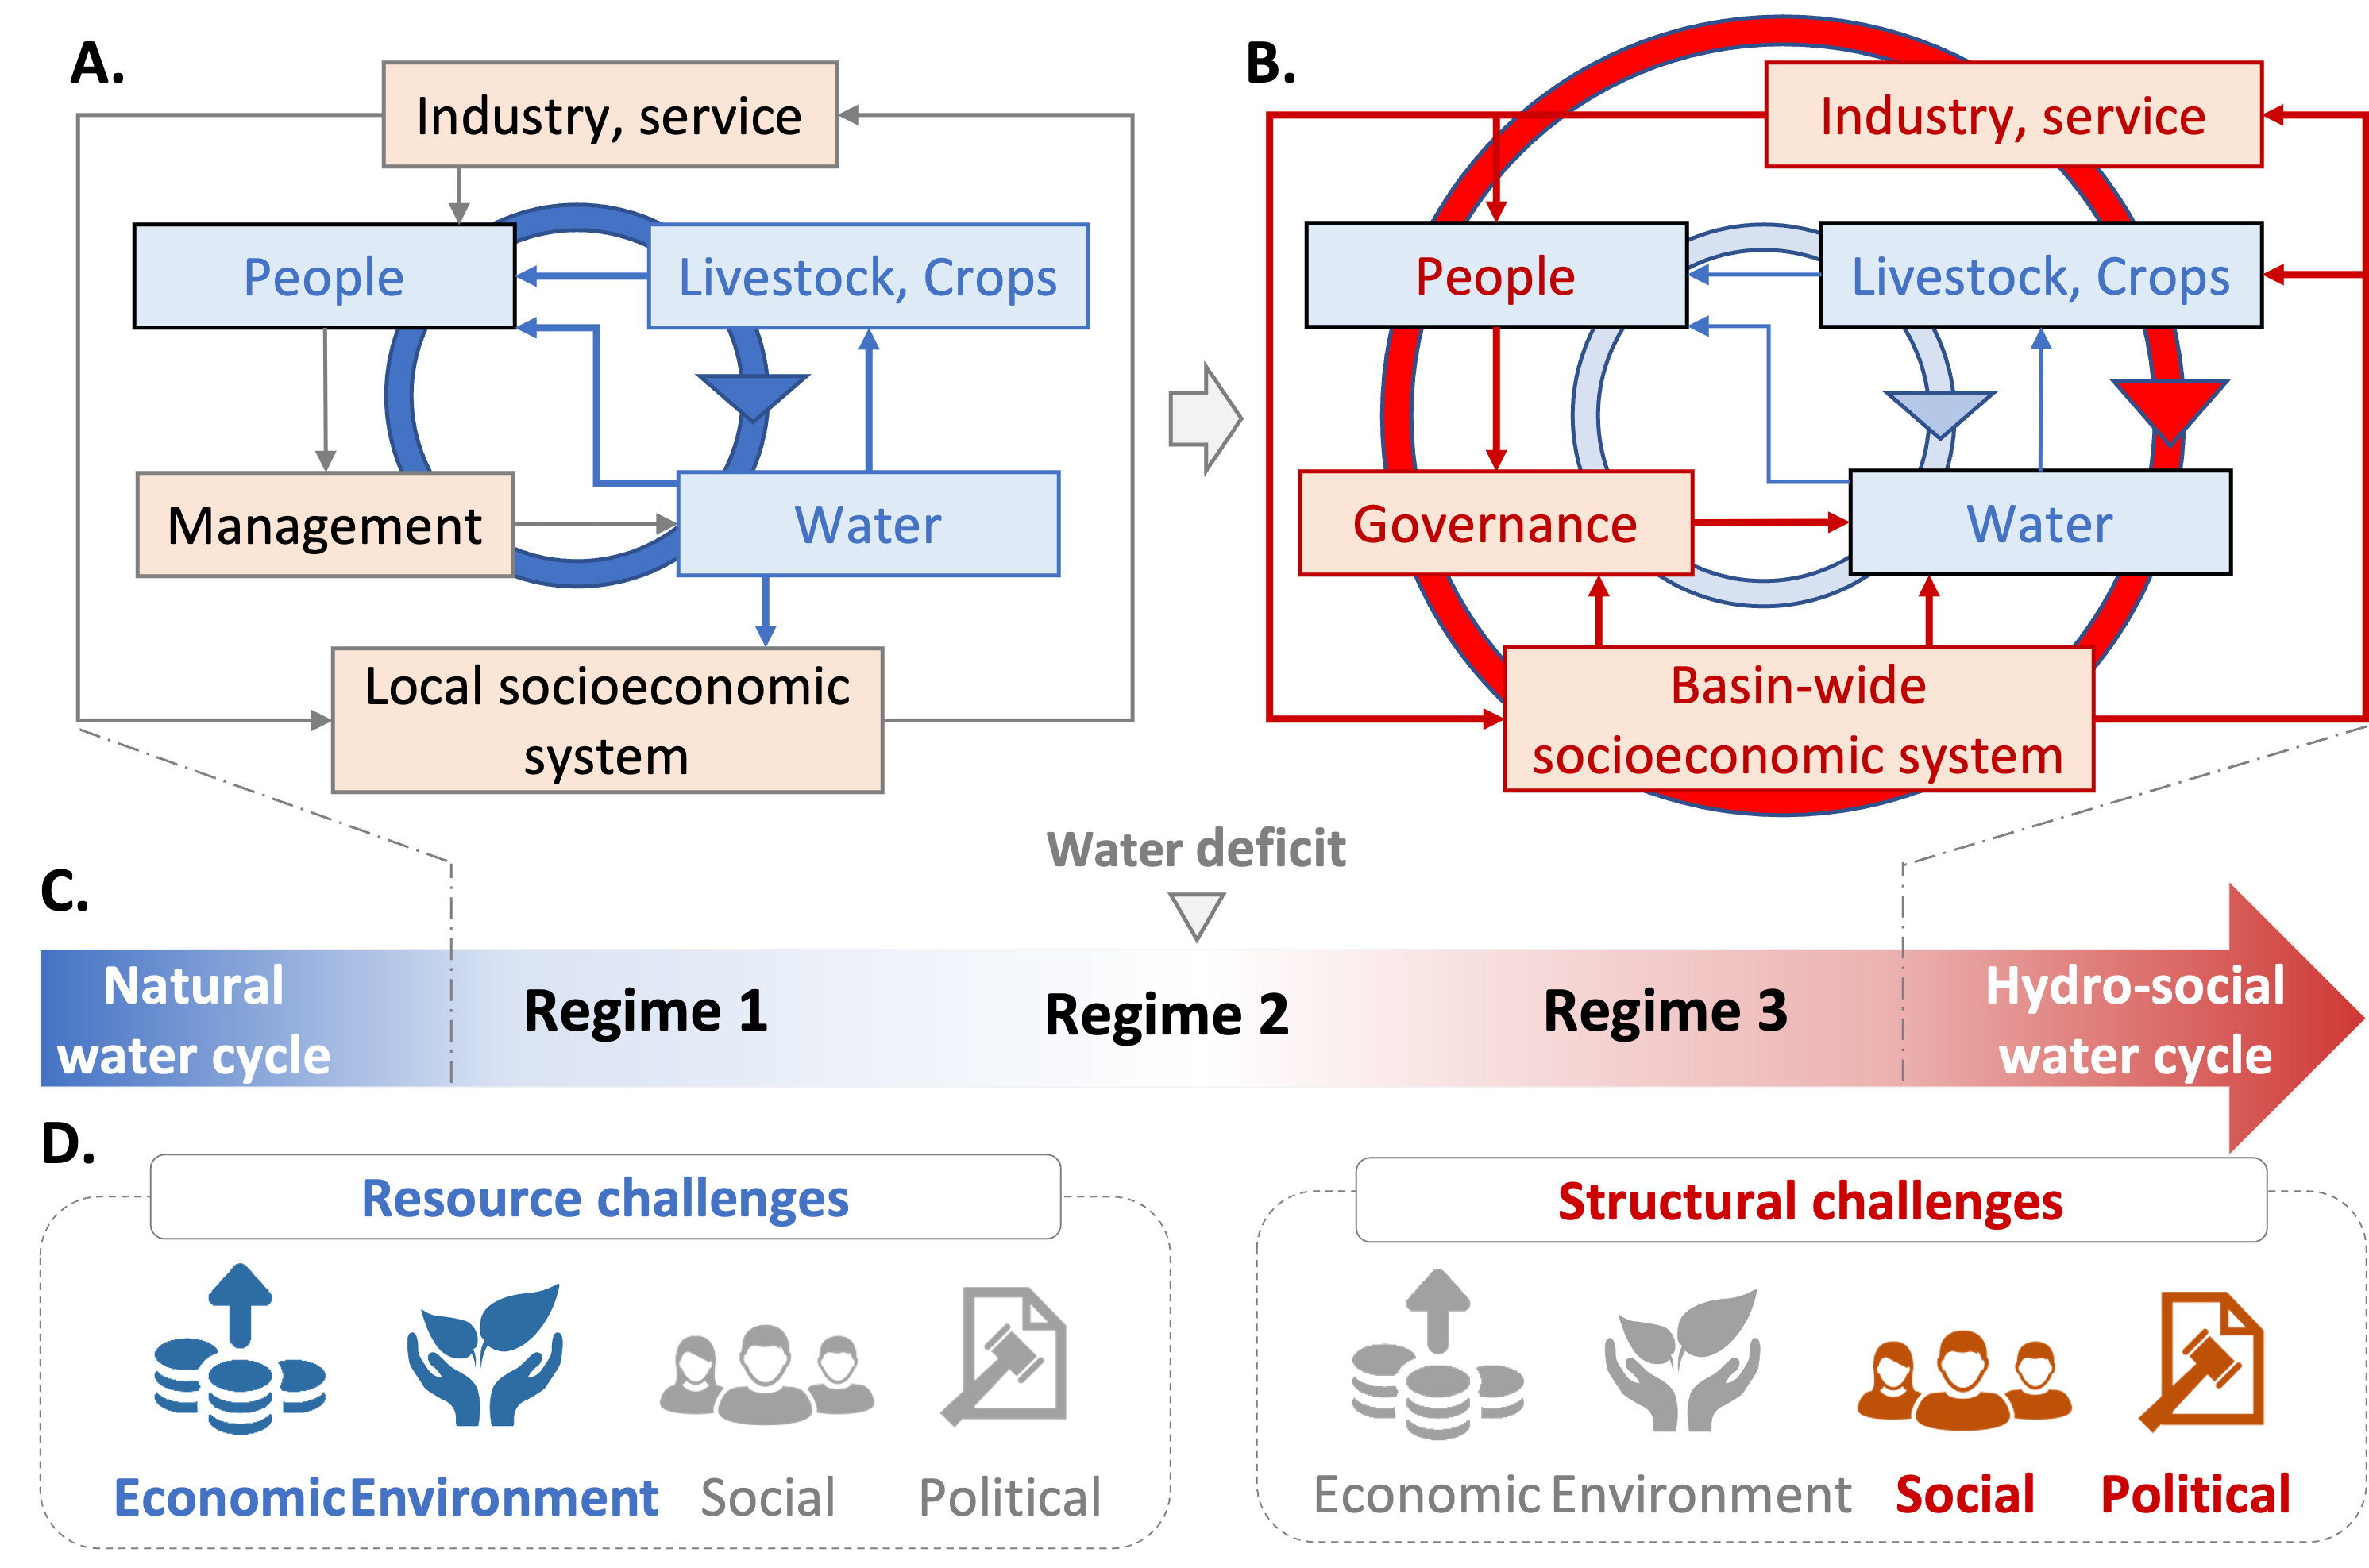
\includegraphics[width=0.8\linewidth]{../../figures/main/transition.png}
	\caption{
		Transition schema of water governance during transformation towards a hydrosocial water cycle. Blue pathways are dominated by natural water cycle while red pathways are dominated by socio-economic feedbacks. There is a transformation towards the hydrosocial water cycle where red loop increases.
		\textbf{A. Early phase.} As socio-economic systems develop, industry and services gradually demand increasing amounts of water; at the same time, increasing social organization and technological capacity allow people to manage water resources more intensively, including intensive intervention in the natural water cycle. 
		\textbf{B. Late phase} With further developed and economically efficient industries and services, trade-offs between provisioning-purpose and non-provisioning water use become prominent. Rather than being determined by local socio-economic systems, water withdraws and management are scaled up to the entire basin. 
		Thus, \textbf{C. Transformation from a natural water cycle towards the hydro-social water cycle} occurs in paralleled with a transformation towards a hydrosocial water cycle. This is generally distinguished when water resource limits are reached. The three water governance regimes seen in the YRB are identified along this transition (Regime 1: massive supply regime, Regime 2: purpose-focused regime, Regime 3: many-sided governance regime).
		\textbf{D. Water governance challenges} Through the transitional regimes, water governance faces primarily economic and environmental challenges in the early phase and social and policy challenges in the late phase.
	}
	\label{fig:summary}
\end{figure*}

% 我们为的研究结果表明,黄河流域能被识别为三个明显的稳态。
Our results show that there have been three distinct but sequential governance regimes within the YRB (Figure~\ref{fig:phases}): a massive supply regime (1965-1978), a purpose-focused regime (1979-1993) and a many-sided governance regime (1994-2013). Shifts between these regimes were caused by different environmental, economic, social or political drivers (Figure~\ref{fig:Causes}).
% 值得注意的是,这些多方面的变化随着流域逐步迈向水-社会循环的过程中逐步发生的,且在早期主要带来经济、环境方面的挑战,而后期则带来社会和政策方面的挑战。
It is important to note that each regime occurred gradually, with multifaceted causes, as the basin moves towards a hydrosocial water cycle.
The challenges were primarily economic and environmental at the beginning of the YRB's water governance trajectory and social and policy-related towards the end (Figure~\ref{fig:summary}).

% 第一种时期(1965-1978年),流域经济以农业为主,自然水资源相对丰富,用水治理倾向于为农业提供更多的资源。
During the massive supply regime (1965-1978), the basin economy was mainly dependent on the agriculture and natural water resources were relatively abundant (\textit{SI Appendix} Figure S5); water governance thus tended to supply more resources for agriculture (e.g. by construction of reservoirs and channels). 
% 因为此时社会经济对自然水循环的影响尚且有限,几乎没有保护政策的治理体系鼓励在需供水的地区进行无节制的取水和蓄水,而很少考虑流域的社会公平。
Due to the limited effects of socio-economic feedbacks on this regime, water governance had few protective policies, assumed an unlimited water supply, and took little consideration of the impacts of water use on social equity and the environment 
\cite{zhouDecelerationChinahuman2020}. 
% 近80%的地表水用于供应,黄河在稳态的后半段干涸了.
Since nearly 80\% of surface water was used (mainly for provisioning purposes), the Yellow River dried up during the second half of the regime (\textit{SI Appendix} Figure S7). 
% 随着干旱化的日益严重,造成了湿地萎缩、生物多样性下降等生态问题,呈现出巨大的环境危机。
Ecological issues, such as wetlands shrinkage and declines in biodiversity, emerged as the drying up became more and more serious, leading a huge social-ecological crisis and a significant challenge to existing modes of water governance rigorously 
\cite{wohlfartSocialecologicalchallenges2016}.

% “目的转轨”的开始恰逢中国的“改革开放”,巨大的社会转型使得新兴工业和服务业打破了农业的主导地位,开始争夺水资源。
The start of the purpose-focused regime (1978) coincided with Chinese ``reform and opening-up''.
This huge social transformation led to the emergence of industry and services, broke the dominance of agriculture, and resulted in higher competition for water use (Figure~\ref{fig:Causes} and \textit{SI Appendix} Fig. S8). 
% 面对遗留的环境问题和全新的经济挑战,黄河水利委员会进行了改组,接到水利部(原水电部)的指示,恢复和加强黄河水利委员会的水文、流域管理工作。
In the face of ongoing environmental challenges and new economic challenges, the Yellow River Conservancy Commission (\textit{SI Appendix} Methods S1) underwent a reorganization and received instructions from the Ministry of Water Resources (then called the Ministry of Water Resources and Electric Power) to resume and strengthen work on hydrology and basin management in the YRB 
\cite{yellowriverarchivesOrganizationalHistoryYellow2004}.
% 在全国率先出台了新的政策法规(如“87调水方案”)进行调水,成功阻止了灌溉用水量的扩大。
As a result, new policies and regulations (e.g., ``the 87 Water Allocation Scheme'') were introduced in the YRB ahead of the rest of the country to allocate water for stopping the expansion of water consumption 
\cite{wang2018}.

% 直到大约1993年以来,由于社会经济发展后先进技术的广泛应用,水资源利用效率有了显著提高,才出现了下一个政权向全面治理的转变。
The next shift, to the many-sided governance regime, did not occur until a significant increase in water use efficiency in about 1993, overcame some resource limits  
\cite{liuWaterconservancyprojects2013}. 
% 区域和部门之间在水需求方面的社会经济权衡在这一制度中发挥关键作用,因此水治理需要满足更全面、更有效率的水分配
Since socio-economic trade-offs between water-dependent regions and sectors played a more important role at this regime, water governance had to achieve efficient water allocation while balancing different purposes in the face of limited water supply  
\cite{dalinBalancingwaterresource2015}.
% 因此,这一时期开始推广的水权转换项目,可以为其他地区的工业发展节约区域农业用水。
For example, the water rights conversion project that has been popularized during this regime may even save regional agricultural water for industrial developments in other regions, and water transfer has been another huge project to meet water demands within the YRB
\cite{barnett2015,yunpeng2010}.
% 但是曾帮助流域摆脱环境危机的分水政策却在此时期成为了流域协调和社会公平的桎梏。
On the other hand, the old water policy (e.g., ``the 87 Water Allocation Scheme''), which once helped the YRB resolve its environmental crisis, limited social equity and coordinated allocation under the new regime because of path dependence 
\cite{wang2018}.
% 类似的,此稳态下国家层面的水治理政策都在进行补充或调整,因为这种制度的缺失和社会的不公平正成为流域新的治理挑战。
Many national-level water policies were proposed or adjusted under this regime, as the absence of such policies and social injustice in water use became new structural challenges for governance
\cite{konarExpandingScopeFoundation2019}.

% 一般来说,在向水社会循环的转变过程中,三种治理制度之间的转变是依次发生的。
In general, shifts between the three governance regimes occurred sequentially during a transformation towards the hydrosocial cycle.
% 随着越来越多的人为影响逐渐改变世界,对生态系统动力学从生物物理控制向社会和政治控制的转变可能在社会-生态系统中变得越来越普遍
Transition from biophysical control to social and political control of ecosystem dynamics may become increasingly widespread in social-ecological systems as increasing anthropogenic impacts gradually change the world  
\cite{bestPaceHumanInducedChange2020,cummingLinkingEconomicGrowth2018,cummingImplicationsAgriculturalTransitions2014}.
Some implications of this kind of change, when accompanied by engineering solutions, have been explored in the Millennium Assessment’s `Technogarden' scenario 
\cite{millenniumecosystemassessmentprogramEcosystemshumanwellbeing2005}.
% 流域转向社会-水循环的过程就是典型的社会-生态系统过渡过程,而我们发现在这一过程中水治理的稳态转换呼应了全球水治理面临的两大主要挑战。
The transition regimes identified here echo the two kinds of major water governance challenges globally (resource challenges and structural challenges, Figure~\ref{fig:summary} and \textit{SI Appendix} Fig. S9)
\cite{singh2019,porcher2019}.
% 以水资源短缺和供水困难为代表的资源挑战,主要是未开发和正在开发的流域所面临的,与经济和环境变化密切相关。
Resource challenges, represented as water shortage and water supplying difficulties, are mainly faced by undeveloped and developing basins and are highly related to economic and environmental changes
\cite{allan2019,florke2018,liuWaterSustainabilityChina2012}. 
% 另一方面,高度控制和发达的流域主要面临结构性挑战,迫切需要在社会政策方面进行协调与合作(如水资源纠纷和缺乏合作治理,特别是跨界河流)。
Alternatively, highly-controlled and developed basins (especially for transboundary rivers) must mainly resolve structural challenges, such as water disputes or lack of equity, and may be in urgent need of novel flexible, efficient sociopolitical governance structures 
\cite{kitroeff2020,roobavannan2017,unep-dhiTransboundaryRiverBasins2016}.
% 非常具有代表性的是,这两类主要挑战在黄河流域快速变迁的过程中先后发生了,伴随着整合了四个维度的(经济、环境、社会、政策)治理稳态的转换。
It is typical that resource challenges and structural challenges have occurred sequentially during the transition of water governance within the YRB. 
% 我们的分析表明,过渡的前期常常带来环境和经济层面的治理挑战,而在过渡的后期则主要是社会和政策层面的挑战。
Our analysis thus suggests that the initial phase of transition often leads to resource-focused challenges that result from economic, demographic and environmental change; while later phases are dominated by structural challenges relating to social and political aspects of governance.
% 再一次,我们总结的框架呼应了联合国发展属为水治理提出的四个维度和两大主要问题。
From the perspective of the core dimensions emphasized by the UNDP for water governance, our proposed schema connects governance challenges and the transformation of large river basins towards a hydrosocial water cycle. 

% 随着河流流域在不同制度之间的过渡而发生的升级过程也带来了额外的挑战。在经济力量的影响下,水资源利用逐渐从一个地方性的问题转变为国家或国际的问题,大型河流流域成为生态系统服务、经济发展和人类福祉的重要来源。
Additional challenges are raised by the process of upscaling that occurs as river basins transition between regimes. Under the influence of economic forces, water use gradually changes from being a primarily local concern to becoming a national or international concern, with large river basins being critical sources of ecosystem services, economic development, and human wellbeing. 
% 例如黄河小浪底调水调沙的生态系统治理需要造成下游河道迅速下切,使农民长期无法从河道中取到灌溉水资源。
For example, the requirement in the ecological system management of water and sediment diversion in the Xiaolangdi Dam of the Yellow River leads to rapid cutting of the downstream river, which makes it impossible for farmers to get irrigation water resources for a long time 
\cite{kongEnvironmentalimpactassessments2017}.
% 通过升级过程成功地引导水况过渡,需要在治理机制中进行相应的升级,并创建能够调节和管理跨规模效应的更高级别机构。
Successful navigation of water regime transitions through an upscaling process requires a corresponding upscaling in the governance regime and the creation of higher-level institutions that can regulate and manage cross-scale effects 
\cite{cummingQuantifyingSocialEcologicalScale2020}. 

\subsection*{Implications and future directions}
\label{Outlook}

% IWGI指数以一种相对简单但全面的方式概括了水管理的过渡制度。
The IWGI index captures the transitional regimes of water governance in a relatively simple but comprehensive way.
% 对科学家和决策者来说,认识到不断变化的治理挑战是重要的,因为发展并不是解决所有与可持续性有关的流域问题的万能药
It is important for scientists and decision makers to recognize the changing governance challenges, because development is not a panacea for all basin issues regarding sustainability 
\cite{cummingLinkingEconomicGrowth2018,reyersSocialEcologicalSystemsInsights2018}.
% 在一种制度下开发的模型和方法在另一种制度下不一定有用。
Models and approaches developed under one regime are not necessarily useful under a different regime.
% 就当今世界而言,与水有关的挑战仍是我们在实现可持续性方面取得进展的主要差距之一,而发展优先战略在许多地方仍是主导方针,可能不利于改善治理
For today's world, water-related challenges remains one of the major gaps in our progress towards sustainability, while development-first strategies are still a dominant guideline in many places and may be in opposition to improving governance 
\cite{xu2020,liu2017,greveGlobalAssessmentWater2018}. 
% 虽然大多数大型河流流域随着发展而在水管理技术和水利用效率方面有所改善,但淡水利用仍被认为正在接近人类-水系统可能崩溃的行星边界
Although most large river basins have shown improvements in water management technologies and water use efficiency along with development, freshwater use is still considered to be approaching planetary boundaries where human-water systems may collapse 
\cite{li2020a,degraafEnvironmentalflowlimits2019,huggins2020}.
% 总的来说,这种明显的治理失败可能有两个主要原因。
Overall, there are probably two main reasons for this apparent failure of governance.
% 首先,农业灌溉效率的显著提高通常伴随着灌溉面积的重新扩大,导致水资源压力的趋势不减(效率悖论)
First, significant improvement in agricultural irrigation efficiency is usually accompanied by a re-expansion of irrigated area, resulting in an unabated trend of water resources stress (the paradox of efficiency) 
\cite{grafton2018}. 
% 其次,如果没有成功的治理,以水循环为主导的复杂治理结构可能会导致流域尺度上水资源使用的灵活性降低,破坏社会-生态系统的恢复力
Second, without successful governance, complicated governance structures dominated by hydrosocial water cycles may result in less flexible water use and undermine the resilience of social-ecological systems at a basin scale
\cite{qinFlexibilityintensityglobal2019,levia2020,grill2019}.
% 从这些角度来看,我们需要更好、更全面的策略来应对治理挑战,因为核心问题是复杂而难以管理的
From these perspectives, we need better and more comprehensive strategies to address governance challenges because the core problems are complex and difficult to manage 
\cite{steffen2020,muneepeerakul2020,bodinCollaborativeEnvironmentalGovernance2017,biermann2012}. 
% 更深入地了解包含非线性变化、制度和过渡思想的治理,应该有助于将治理的重点转移到维持流域社会-生态系统的恢复力和提高其可持续性。
A deeper understanding of governance that incorporates ideas of non-liner change, regimes, and transitions should help to shift the focus of governance towards maintaining the resilience of the basin’s social-ecological system and improving its sustainability.

%tag 研究方法
\matmethods{
We constructed the Integrated Water Governance Index (IWGI) based on three dimensions (supply, purpose, allocation, see Figure~\ref{fig:framework}) and identified the changes periods of the index over time by change points detection. 
Each dimension is reflected by an independent indicator after normalization, and water governance regimes were characterized by the combination of impacts along each dimension at different time periods.
The contribution to changes of IWGI index along with each main indicator were also decomposed and calculated separately for each regime period. 
	
	\subsection*{Integrated Water Governance (IWGI)}
	% 我们认为水资源利用制度,与水资源利用的三个维度紧密相关:
	Water resources governance system is closely related to a transformation towards a hydrosocial water cycle in the three dimensions below (see Figure~\ref{fig:framework} and \textit{SI Appendix} Methods S4 for details)
	\cite{steffen2018,abbottwatercycleAnthropocene2019,levia2020}:
	
	% - 社会的发展通常伴随着用水向社会经济系统倾斜,用水方式优先向收益更高的非供给性方式倾斜:
	\begin{itemize}
		% - 可持续的社会发展应该通过技术手段有效缓解发展过程中产生的水资源压力,才能实现可持续发展:
		\item \textbf{Supply($S$)}: Socio-economic dominance may lead to further demands on the water supply because of increasing water withdrawals. However, since effective water governance may boost supply capacities to meet water demands by technical solutions in the process of development: 
		$$ Transformation \propto S^{-1} $$

		\item \textbf{Priority($P$)}: Transformation is usually accompanied by a change of purpose in water governance towards socio-economic services (usually towards non-provisioning purposes), because of higher returns:
		$$ Transformation \propto P $$

		% - 社会发展通常伴随着更具结构性的水资源配置,如区域部门之间的分工合作,以及区域的统筹配置:
		\item \textbf{Allocation($A$)}: Transformation usually leads to more complicated structures in water allocation, as a result of division and cooperation between regions and sectors because of environmental context and economic comparative advantages:
		$$ Transformation \propto A $$ 

	\end{itemize}
	
	% 将三者合一起,即:
	We combined these three dimensions into a single integrated index, keeping their positive or negative relationship with the transformation towards a hydrosocial water cycle: 
	
	$$ Transformation \propto P*A*S^{-1}$$

	% 在上述假设的基础上,我们要构建流域综合耦合指数(Integrated Water Resources governance, IWGI),使 IWGI 有效表征与用水相关的三个维度。首先为每个维度选择一个合适的指示因子(indicator, $I_x$, 其中$x=P, C or S$)。将上式进行自然对数转换,从而让三个维度之间变成加减关系:
	To effectively represent the three dimensions, we selected an appropriate indicator ($I_x$, $x=S$, $P$ or $A$ corresponding to supply, purpose, and allocation respectively) for each dimension. Then, the above equation was transformed into a natural logarithm to facilitate calculation:

	$$ Transformation \propto ln(I_S) + ln(I_P) - ln(I_A) $$

	Assuming they have equal weights, the Integrated Water Governance Index (IWGI) is:

	$$ IWGI = I'_S + I'_P - I'_A $$

	where $I'_x$ is a normalization of log-transformed indicator $I_x$ for a certain dimension:

	$$ I'_x = normalize(ln(I_x)) $$
	
	\subsubsection*{Normalization}
	We tested different normalization methods, and they made no difference in change points detection (see \textit{SI Appendix} Methods S5. Sensitivity analysis). We performed min-max normalization using the formulation below:

	$$ normalize(X) = (X - X_{min}) / (X_{max} - X_{min}) $$

	\subsubsection*{Indicator of supply}
	We used the scarcity-flexibility-variability (SFV) water stress index proposed in Qin et al., 2019 to evaluate water supply capacities ($SFV_i$) as the indicator in a certain region $i$ \cite{qinFlexibilityintensityglobal2019}. This metric takes into account management measures (such as the construction of reservoirs) and the impact of changes in the industrial structure of water use on the evaluation of water scarcity (see \textit{SI Appendix} Methods S4 for details). For the whole YRB, the indicator of supply capacity $I_S$ is the average of all regions' SFV-index: 

	$$ I_S = \frac{1}{4} * \sum_{i=1}^4 SFV_{i} $$
	
	Where $SFV_i$ is the SFV-index for region $i$, and $i=1$ to $4$ refers SR, UR, MR, and DR (see \textit{SI Appendix} Methods S1 Definition of study area).

	\subsubsection*{Indicator of purpose}
	To quantify purpose $I_P$, we used Non-Provisioning purpose Shares (NPS) of water use as an indicator. While provisioning purpose water use ($WU_{pro}$) includes domestic, irrigated and livestock water uses, non-provisioning purpose water use ($WU_{non-pro}$) includes industrial and urban services water uses. We calculated the NPS as:

	$$ NPS_{i} = \frac{WU_{non-pro, i}}{WU_{pro, i} + WU_{non-pro, i}} $$

	Where $i$ refers a certain region, or the whole basin, i.e:

	$I_P$ = $NPS_{basin}$

	\subsubsection*{Indicator of allocations}
	%$AEM$ 指标度量的是水资源配置“不均匀”的程度,类似于信息熵是对“混乱程度”的度量,即参与分配的各个单位之间,分配比例差距越大,则熵越小。
	% 而我们的指标应反映随着社会发展,水资源配置在区域之间更加均衡(比例差距小)、整体满足不同用水部门的发展需求(比例差距减小)、但不同区域存在部门分工(比例差距增大)的趋势。
	To describe allocations $I_C$, we designed an indicator based on information entropy, called Allocation Entropy Metric (AEM), AEM measures the degree of evenness of water allocation (see \textit{SI Appendix} Methods S4).
	Our indicator $I_C$ was intended to reflect the idea that with the development of society, water resources allocation becomes more balanced among regions and generally meets the needs of different sectors, but different regions have a trend of division of labour among various sectors (with larger gaps):

	$$ I_C = \frac{AEM_{r}*AEM_{s}}{AEM_{rs}}$$
	
	where $AEM_{r}$ and $AEM_{s}$ are Allocation Entropy Metric in different regions and different sectors. $AEM_{rs}$ describes differences between sectors in a certain region relative to the whole basin (see \textit{SI Appendix} Methods S4). 

	\subsection*{Change points detection}
		% The method makes no assumptions about the distribution of the data and detects breakpoints based solely on the probability of the data coming from different distributions before and after the breakpoint.

		With no assumptions about the distribution of the data, the Pettitt (1979) approach of change-point detection is commonly applied to detect a single change-point in hydrological time series with continuous data \cite{pettittNonParametricApproachChangePoint1979}. 
		It tests $H0$: The variables follow one or more distributions that have the same location parameter (no change), against the alternative: a change point exists. The non-parametric statistic is defined as:
	
		$$ K_t = max|U_{t, T}|$$

		Where:

		$$ U_{t, T} = \sum_{i=1}^t\sum_{j=t+1}^T sgn(X_i - X_j) $$
	
		The change-point of the series is located at $K_T$, provided that the statistic is significant. We used 0.001 as the threshold p-value (see \textit{SI Appendix} Methods S5 for Sensitivity analysis), meaning that the probability of a statistically significant change-point judgment being valid was more than $99.9\%$.
		Since this method can only return one significant change point, we repeated it until all significant change points were detected.
	
	% 计算贡献度
	\subsection*{Contribution decomposition}
		We decomposed the amount of variation in each index at different periods in order to quantify the contribution of each influence to the index. Using the Integrated Water Resources governance (IWGI) Index as an example, its value is influenced by normalized indicators in three dimensions: stress ($I'_S$), purpose ($I'_P$) and allocation ($I'_C$). We can calculate their differences between two certain years ($y_2$ and $y_1$, $y_2 > y_1$) by:

		\begin{align*}
			\Delta IWGI &= (I'_{P_{y_2}} + I'_{C_{y_2}} - I'_{S_{y_2}}) - (I'_{P_{y_1}} + I'_{C_{y_1}} - I'_{S_{y_1}}) \\
			&= (I'_{P_{y_2}} - I'_{P_{y_1}}) + (I'_{C_{y_2}} - I'_{C_{y_1}}) + (I'_{S_{y_1}} - I'_{S_{y_2}}) \\
			&= \Delta I'_P + \Delta I'_C + (-\Delta I'_S)
		\end{align*}
		Then, the contribution of dimension $x$ to IWGI's changes can be referred as:

		$$ Contribution_x = \frac{\Delta I'_x}{|\Delta IWGI|} $$

		% Since $Contribution_x$ can be positive or negative, we used an absolute value to evaluate the contribution (in proportion) of a certain dimension in the all three dimensions to the changes:
		% $$  Contribution_x\% = \frac{|\Delta I'_x|}{\sum_x |\Delta I'_x|} $$

		% or just for contributions (in proportion) within a certain year $j$ to the regime:
		% $$ Contribution_{x,j}\% = \frac{|I'_{x, j}|}{|\sum_x I'_{x, j}|} $$

	\subsection*{Datasets}
	% 为了计算 IWGI ,我们需要计算多个指标及子指标,所有使用的数据集都在表中列出,数据的详细介绍可见补充材料。
	In order to calculate IWGI, we need to calculate multiple indicators and sub-indicators. All the datasets used are listed in the \textit{SI Appendix} table S1. A detailed description of the data is provided in the supplementary materials \textit{SI Appendix} Methods S2.
}

\showmatmethods{} % Display the Materials and Methods section

\acknow{Funding was provided by the National Natural Science Foundation of China (CN) (Grant Nos. NSFC 42041007).}

\showacknow{} % Display the acknowledgments section

% Bibliography
\bibliography{my-papers}
	
\end{document}